\documentclass[../thesis]{subfiles}

\begin{document}
	\subsection{Results}
	\label{subsec:mic:native:results}

	\tdg{sugar and methodology}
	Although the \intel\xeonphi coprocessor is able to run the same code as a regular \intel\xeon processor, the question remains whether it is able to achieve similar or higher efficiency without extra effort. This section shows the results obtained with performance tests using the diagonal strategy in the coprocessor, following the methodology described in \cref{sec:case:method} with a block dimension of 32.

	\tdg{environment}
	Measurements for this section were performed using a single computational node of the 711 group in the \search cluster, containing two \intel\xeon E5-2670 \cpus sharing 64GB DRAM (\numa) and an \intel\xeonphi Coprocessor 5110P (see \cref{tab:search:711} for the hardware details). These nodes run Linux CentOS 6.4 and provide \intel Composer XE 2013. Tests were built with \icpc 13.1.2, \mkl, and Armadillo (3.900.7).

	\begin{table}[!b]
		\centering
		\begin{tabular}{|l|c|c|}
			\hline
			& \textbf{CPU} & \textbf{MIC}  \\
			\hline
			Clock frequency & 2.60 GHz & 1.053 GHz  \\
			Cores & 8 & 60  \\
			SIMD width & 256-bit (\avx) & 512-bit  \\
			Memory type & --- & \gddr5  \\
			Memory size & 64 GB & 8 GB  \\
			Memory speed & --- & 5.0 GT/s  \\
			\hline
			Peak DP FLOPs & 166.4 GigaFLOP/s & 1.01 TeraFLOP/s  \\
			Peak Memory Bandwidth & 51.2 GB/s & 320 GB/s  \\ 
			\hline
		\end{tabular}
		\caption{Hardware details for \search node 711-1. Further information available in \cite{Intel:Xeon:e5_2670,Intel:Xeon:e5_2600,Intel:XeonPhi:5110P}.}
		\label{tab:search:711}
	\end{table}

	\begin{figure}[t]
		\begin{minipage}{0.48\textwidth}
			\centering
			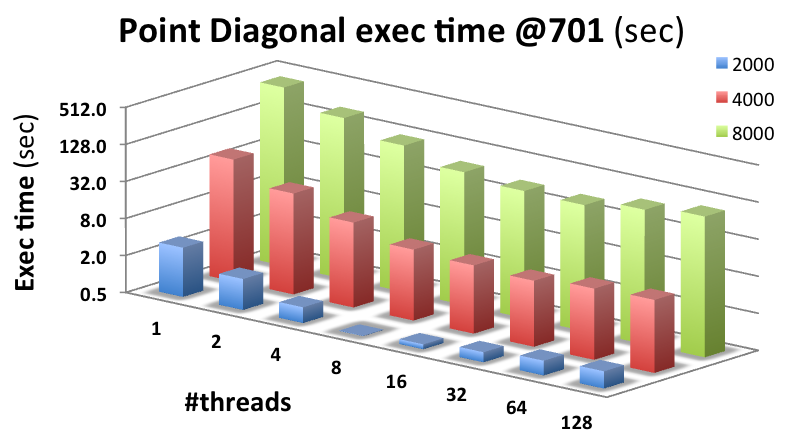
\includegraphics[width=\textwidth]{assets/images/mic/point-diagonal.png}
			\captionsetup{font=small}
			\caption{Execution times for point-diagonal in the \intel\xeonphi}
			\label{fig:mic:point:diagonal:times}
		\end{minipage}
		\hfill
		\begin{minipage}{0.48\textwidth}
			\centering
			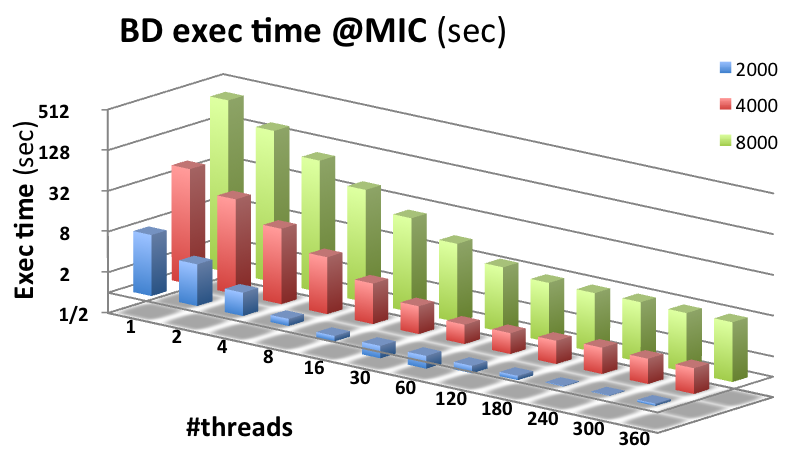
\includegraphics[width=\textwidth]{assets/images/mic/block-diagonal.png}
			\captionsetup{font=small}
			\caption{Execution times for block-diagonal strategy in the \intel\xeonphi}
			\label{fig:mic:block:diagonal:times}
		\end{minipage}
	\end{figure}

	\begin{figure}[t]
		\centering
		\begin{minipage}{0.7\textwidth}
			\centering
			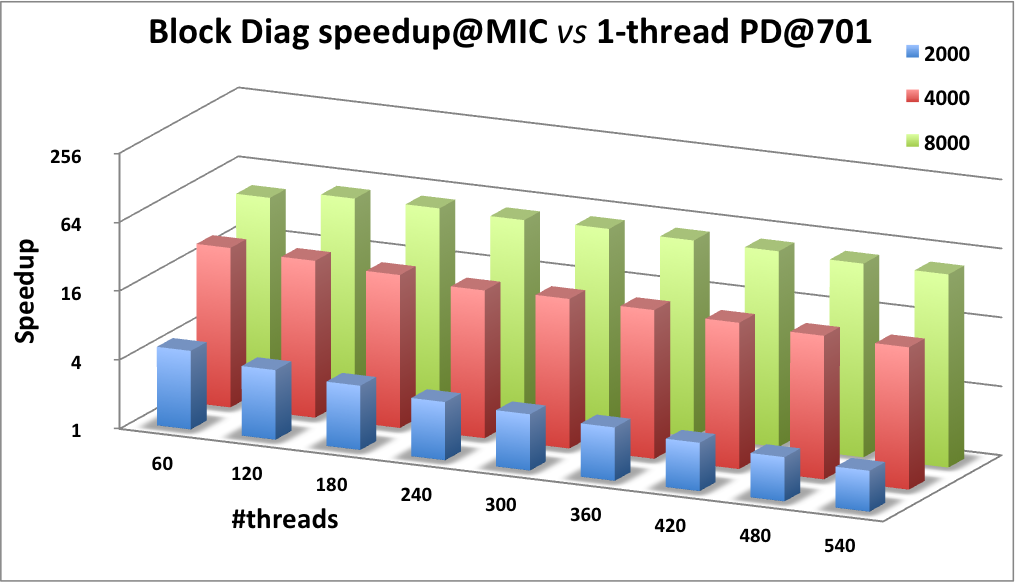
\includegraphics[width=0.8\textwidth]{assets/images/mic/mic-cpu-speedup-accumulated.png}
			\captionsetup{font=small}
			\caption{Accumulated speedup from block-diagonal in the \intel\xeonphi versus point-diagonal in the \cpu.}
			\label{fig:mic:mic-cpu:speedup:accumulated}
		\end{minipage}
	\end{figure}

	\Cref{fig:mic:point:diagonal:times,fig:mic:block:diagonal:times} show the obtained execution times using the diagonal strategy for both methods as described in \cref{chp:multicore}. The scalability of the algorithm is near perfect for both, with the execution time being cut almost by half until the number of threads matches the number of cores in the device. After that, the speedup slows down, with the point method reaching its peak performance when using 4 hardware threads per core (full Hyper-Threading) and the block method plateauing at 2 hardware threads per core. The block method performance only leaves this plateau when 8 or more threads per core are used.
	Although the accumulated speedup of executing the block-diagonal in the \intel\xeonphi is still significant when compared to single-threaded point method in the \cpu, it does not even reach half of the accumulated speedup achieved in the \cpu (\cref{fig:mic:mic-cpu:speedup:accumulated}). In fact, when comparing the accumulated speedups in both platforms, the best value obtained in the \intel\xeonphi is about three times slower than the best value obtained in the \cpu.
\end{document}
